\begin{figure}
    \centering
    \begin{subfigure}{0.45\textwidth}
    	\centering
    	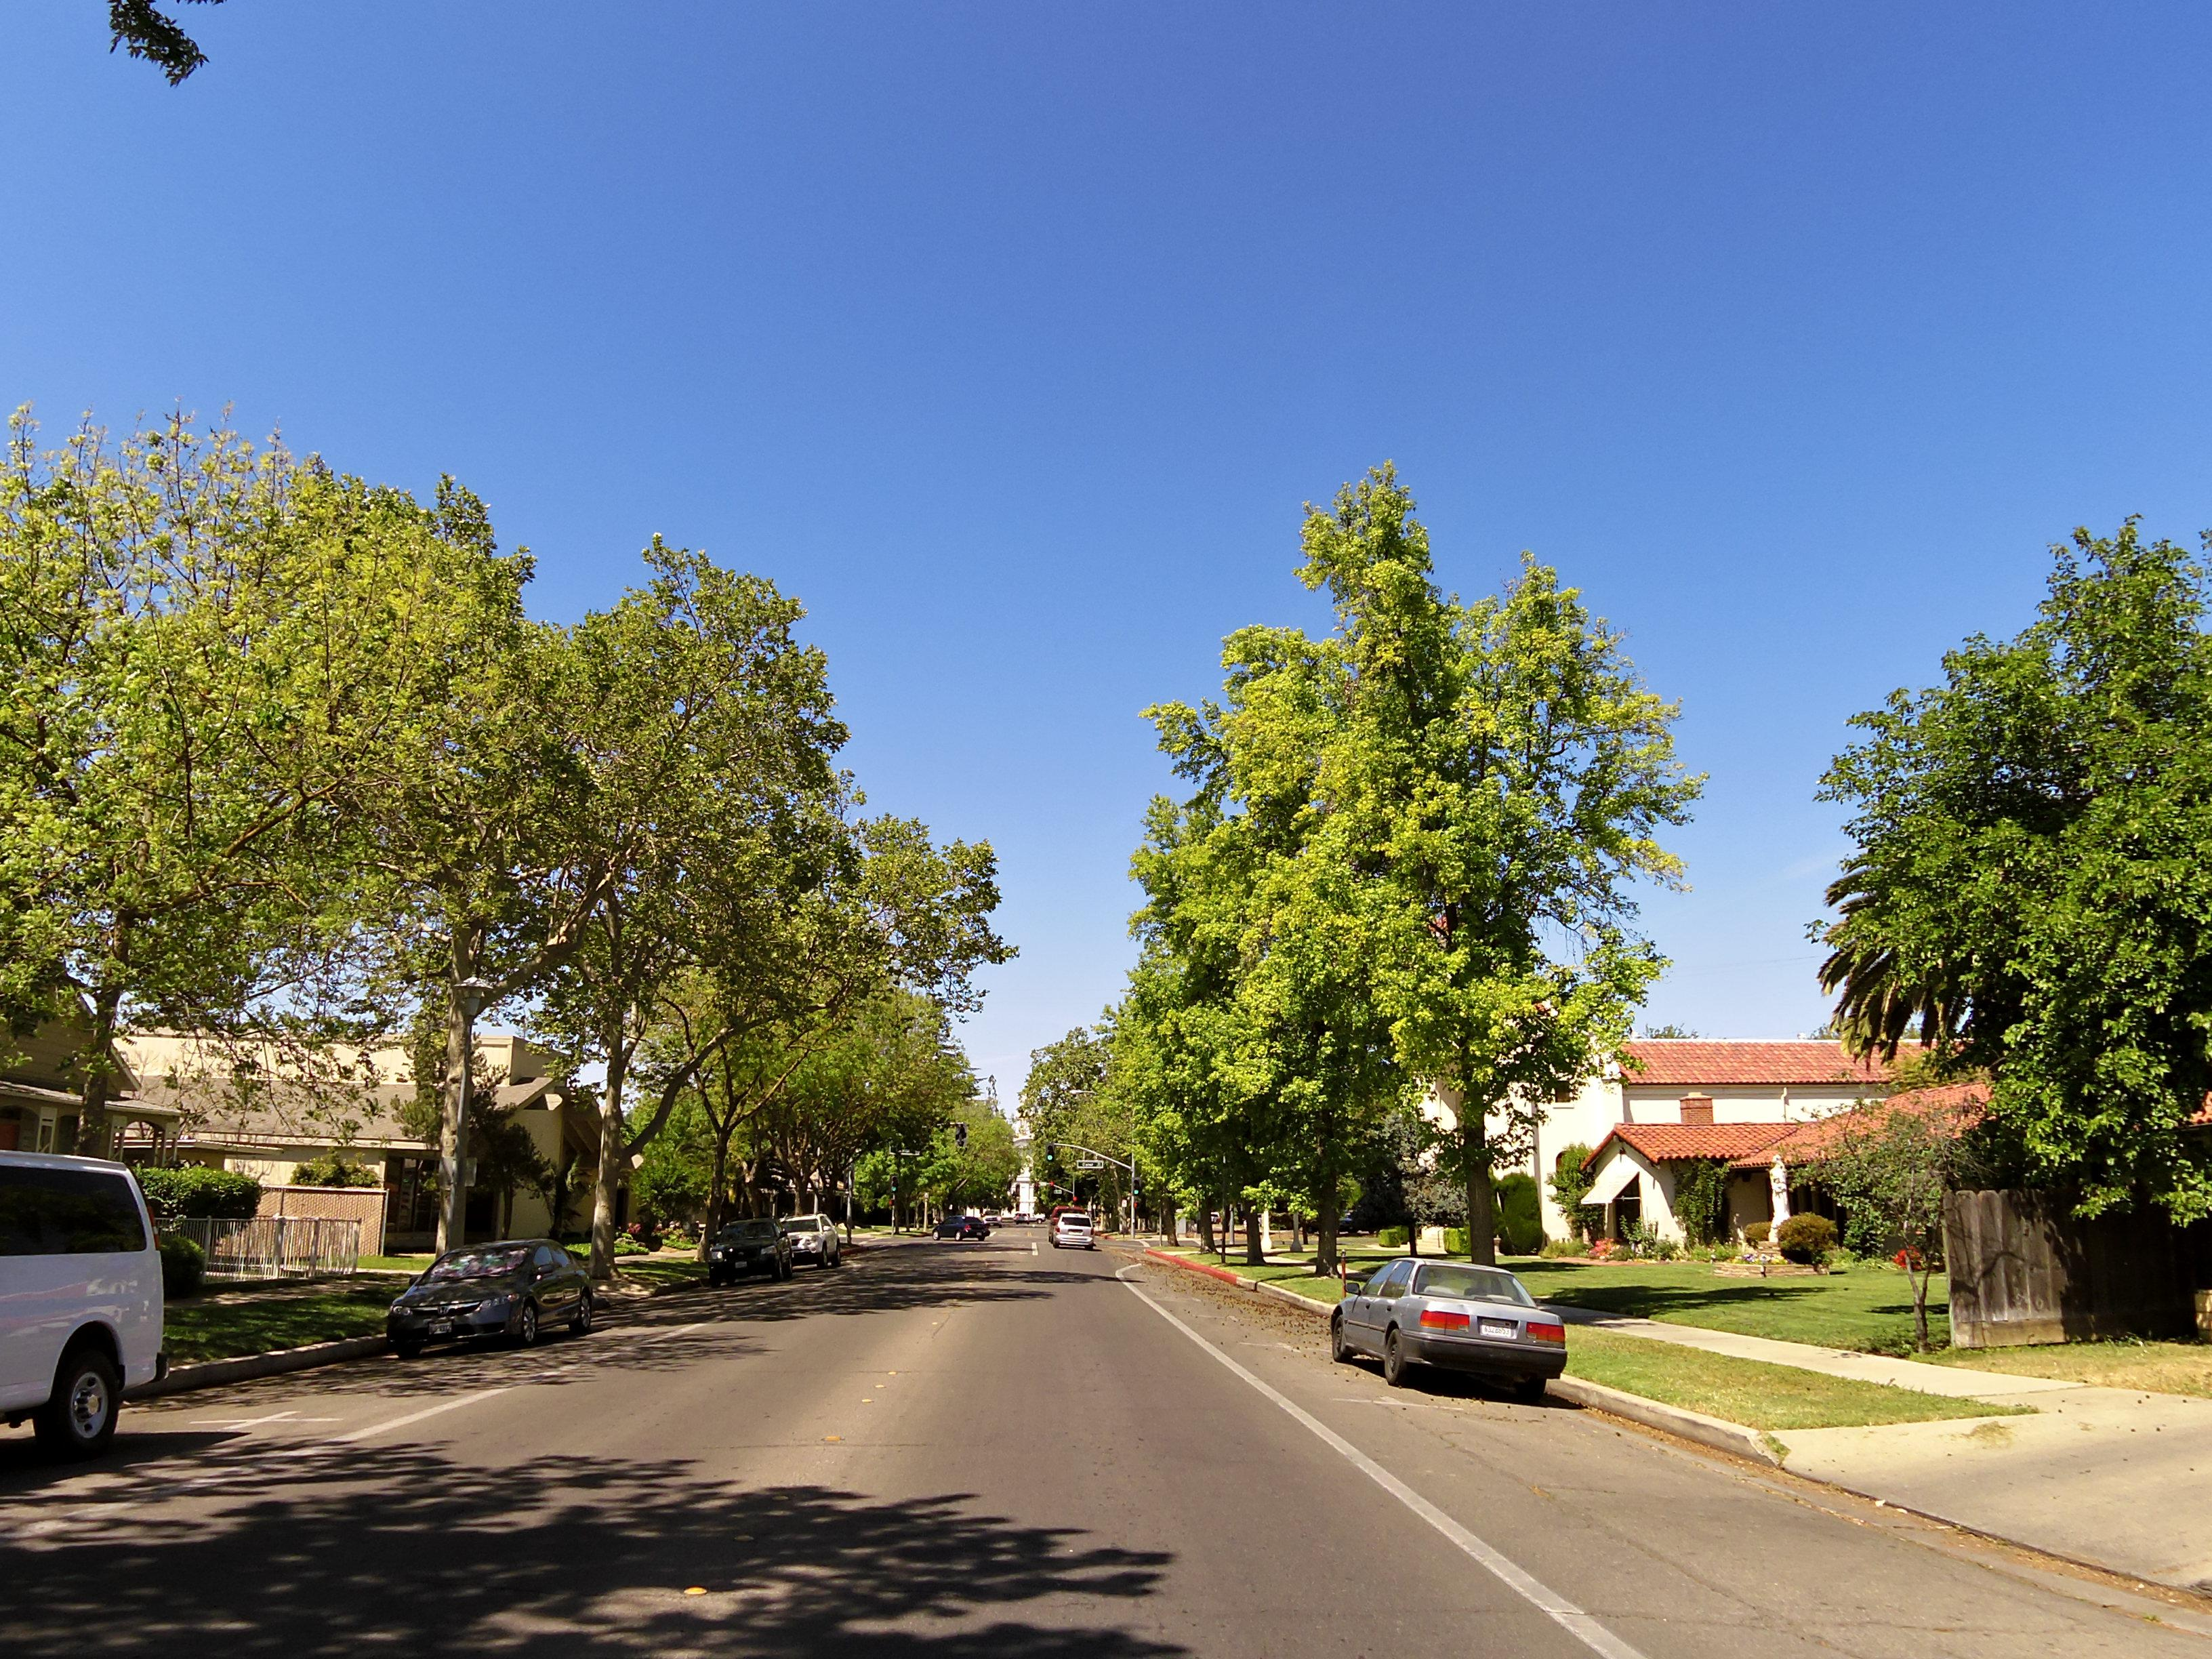
\includegraphics[width=0.9\textwidth]{figures/background/raw.jpg} % first figure itself
    	\caption{An example of a street-level image that is taken using a regular color camera.} \label{fig:background-raw}
    \end{subfigure}
	\hfill
    \begin{subfigure}{0.45\textwidth}
        \centering
        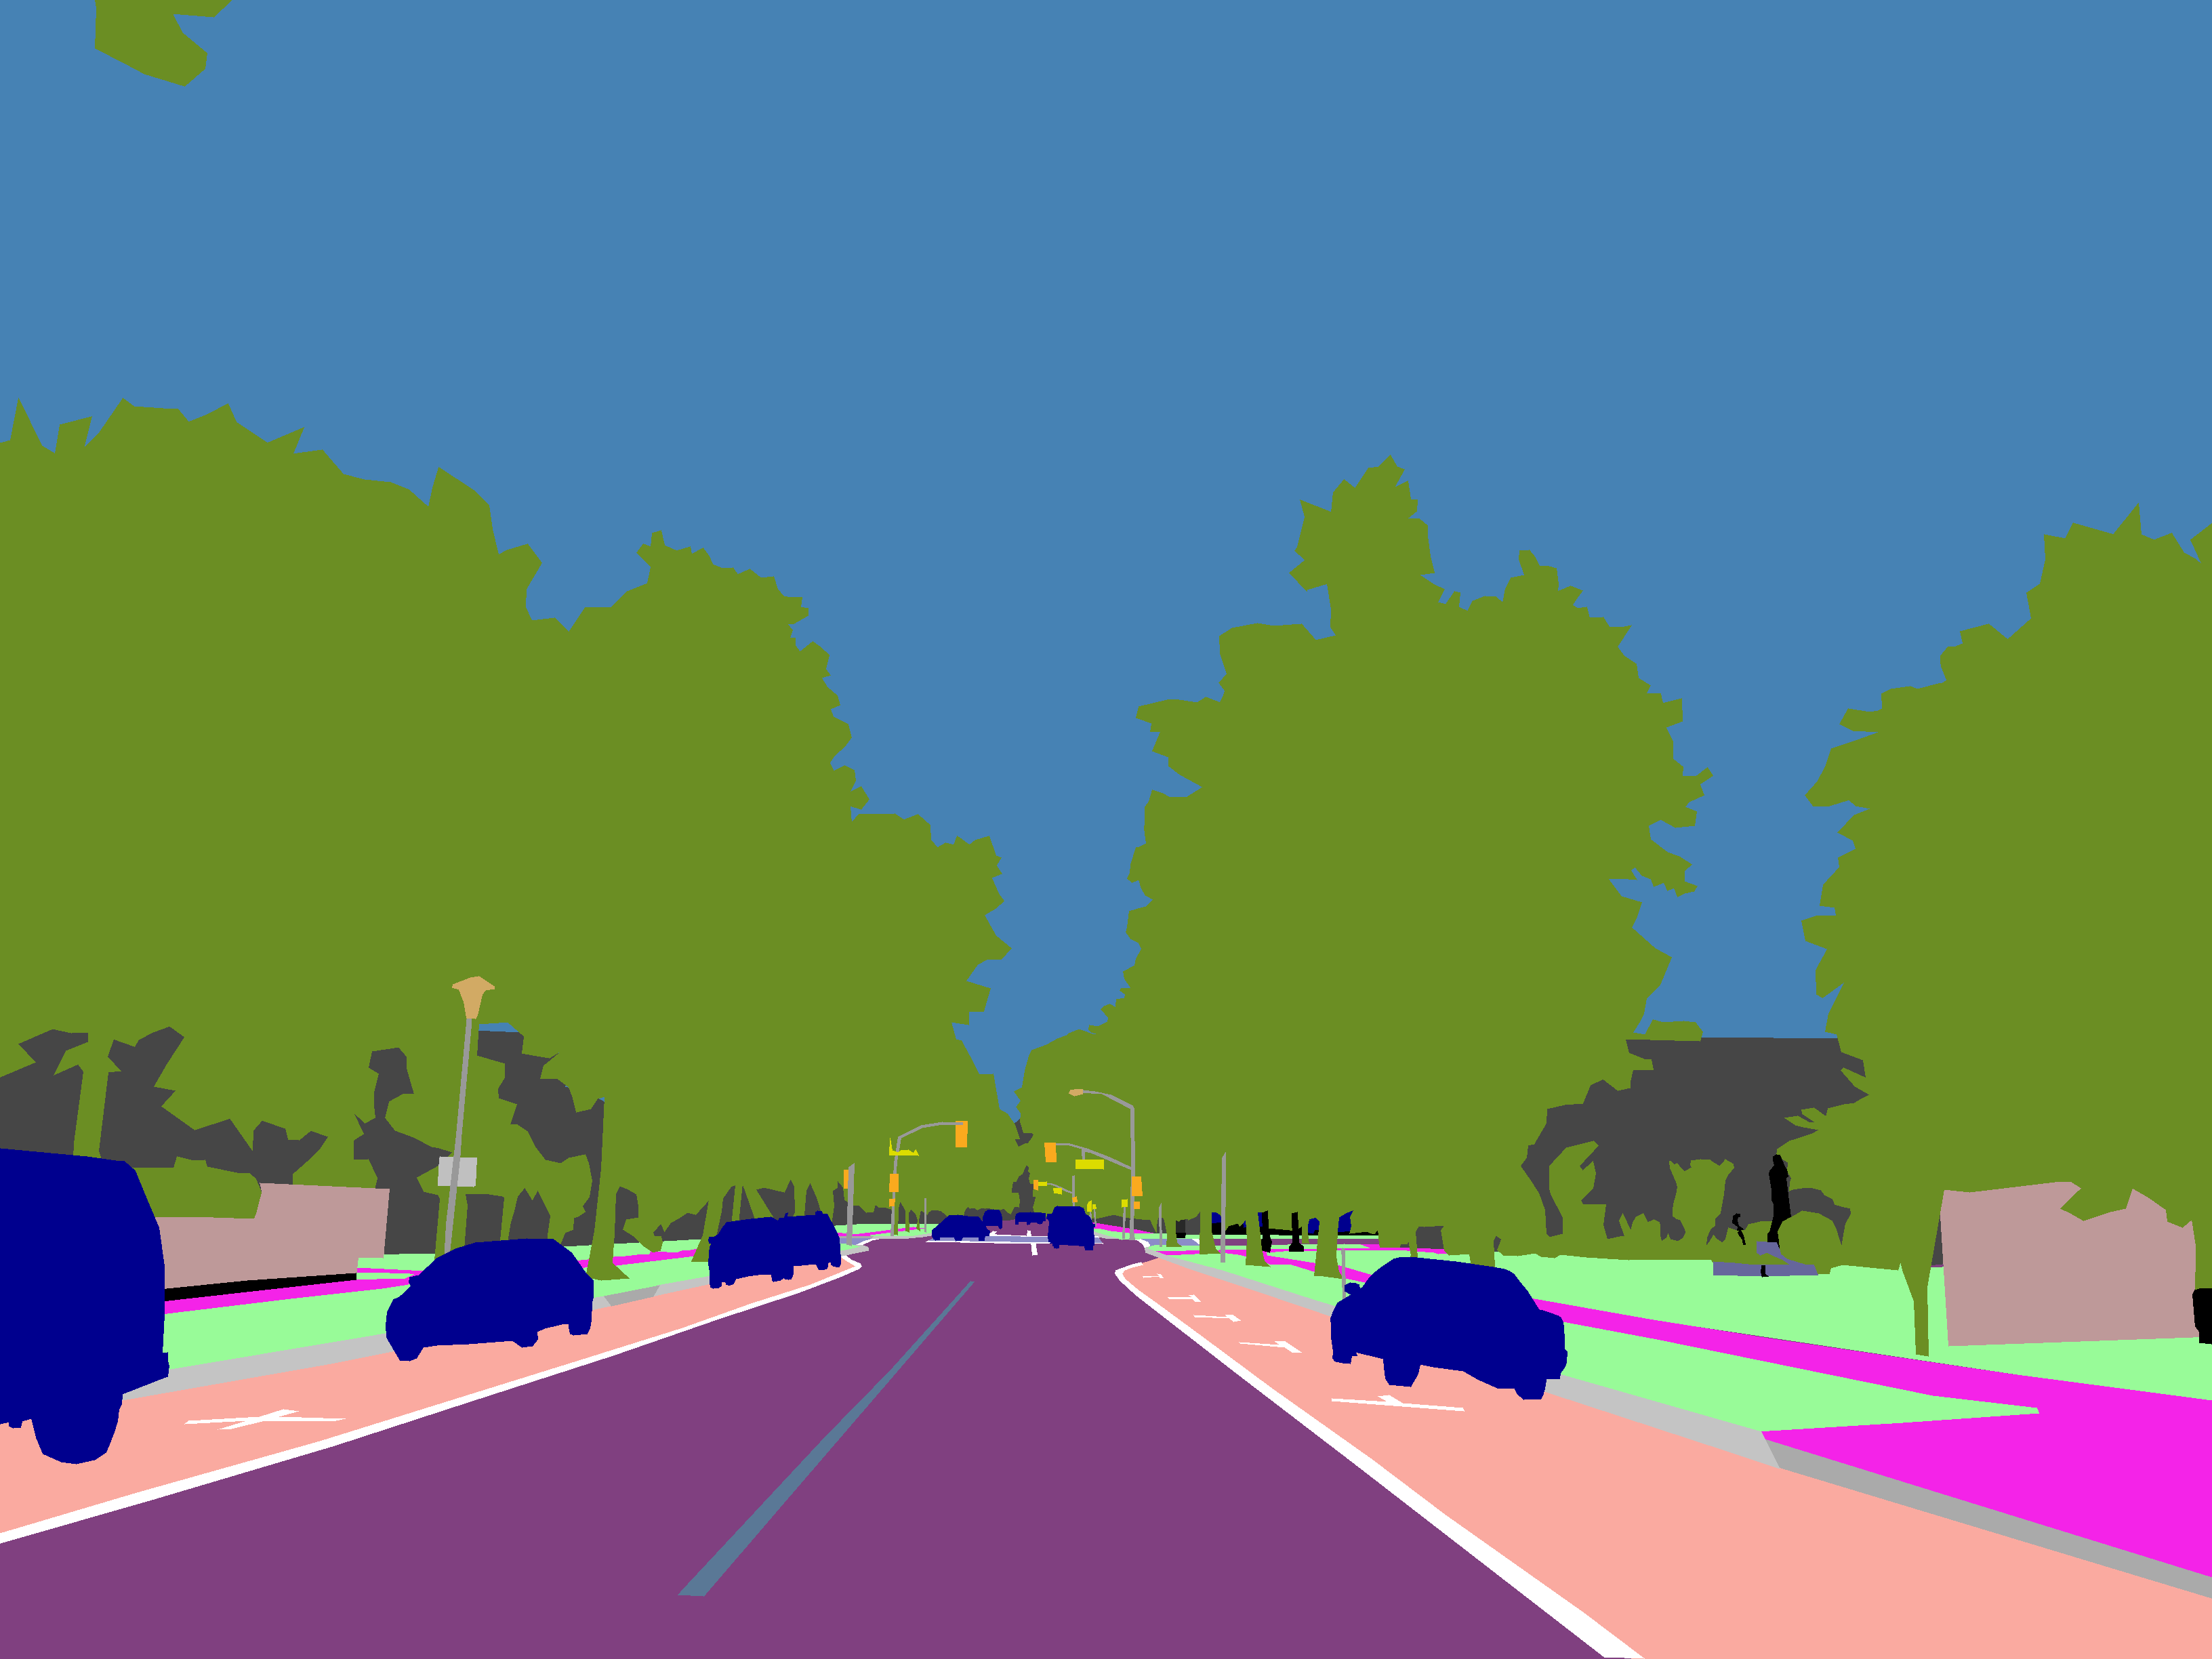
\includegraphics[width=0.9\textwidth]{figures/background/segmented.png} % second figure itself
        \caption{The segmented version of the image, each color representing a different class.} \label{fig:background-segmented}
    \end{subfigure}
	\caption[An example of semantic segmentation.]{An example of semantic segmentation on a color image. This example is taken from the Mapillary dataset~\cite{mapillary}.}
\end{figure}